% LaTeX Article Template - customizing header and footer
\documentclass{article}

\newtheorem{thm}{Theorem}

% Set left margin - The default is 1 inch, so the following 
% command sets a 1.25-inch left margin.
\setlength{\oddsidemargin}{0.25in}

% Set width of the text - What is left will be the right margin.
% In this case, right margin is 8.5in - 1.25in - 6in = 1.25in.
\setlength{\textwidth}{6in}

% Set top margin - The default is 1 inch, so the following 
% command sets a 0.75-inch top margin.
\setlength{\topmargin}{-0.25in}

% Set height of the header
\setlength{\headheight}{0.3in}

% Set vertical distance between the header and the text
\setlength{\headsep}{0.2in}

% Set height of the text
\setlength{\textheight}{9in}

% Set vertical distance between the text and the
% bottom of footer
\setlength{\footskip}{0.1in}

% Set the beginning of a LaTeX document
\usepackage{tikz}
\usepackage{multirow}
\usepackage{fullpage}
\usepackage{graphicx}
\usepackage{amsthm}
\usepackage{url}
\usepackage{amssymb}
\usepackage{amssymb}
\usepackage{algpseudocode}
\graphicspath{%
    {converted_graphics/}% inserted by PCTeX
    {/}% inserted by PCTeX
}
%%%%%%%%%%%%%%%%%%%%%%%%%%%%%




\begin{document}\title{Homework $3$\\ Computer Science \\ B551 Spring 2018\\ Hasan Kurban}         % Enter your title between curly braces
\author{Jinju Jiang}        % Enter your name between curly braces
\date{\today}          % Enter your date or \today between curly braces
\maketitle

      
% Redefine "plain" pagestyle
\makeatother     % `@' is restored as a "non-letter" character




% Set to use the "plain" pagestyle
\pagestyle{plain}
\section*{Introduction}
The aim of this homework is to get you well-acquainted with $\alpha\beta$. You will turn-in two files \begin{itemize} \item A *pdf with the written answers called \texttt{hw3\_jiangjinju.pdf} \item  A Python script called gobblet.py\end{itemize}  I am providing this \LaTeX{} document for you to freely use as well. Please enjoy this homework and ask yourself what interests you and then how can you add that interest to it!  Finally, problems 1 and 2 are worth 20 each and problem 3 is worth 120 points. Include that
statement, ``All the work herein is mine."

\newpage
\section*{Homework Questions}
\begin{enumerate}
\item A general search strategy is to work from both the start and goal--think of navigating a maze. Is this 
a sound strategy for a game? Recall that soundness means $\vdash_{Robot}$\ A $\rightarrow\models_{Human}$ A\\
\underline{Answer to question 1:}\\
The search from both the start and goal is Bidirectional Search,simultaneously search forward from S and backwards from G,stop when both “meet in the middle”,need to keep track of the intersection of 2 open sets of nodes.
Take "navigating a maze" as an example, bidirectional search is a sound strategy since it can find the solution if there is solution, which means if the system is true,$\vdash_{Robot}$\ A, then $\rightarrow\models_{Human}$ A is true.\\
But I have some additional questions about bidirectional search:which to take if there are multiple goal states?where to start if there is only a goal test, no explicit list?
\item Assume there is a game with three players $A,B,C$. You have an evaluation function h that returns
3 numbers: $h(\sigma) =  \langle A_s, B_s, C_s \rangle$ where $\sigma$ is a state of the game and the numbers reflect the goodness
of the state for the respectively named players. In no more than two paragraphs, is there a way to
modify minimax to work with 3 players? Assume that you cannot exhaustively search the game space
and you're able to generate from a state all the next states.\\
\underline{Answer to question 2:}\\
For 3 players, each player is to max his/her goodness, then for each player, we use maximum strategy, here it is the graphs to demonstrate how it works:\\
\begin{itemize}
\item First player. A, choose the maximum $A_s$ from the next states list.
\item Second player, then from Max($A_s$) state's next states, B choose the maximum goodness Max($B_s$) for himself.
\item The third player, choose the Max($C_s$) from the next states of Max($B_s$).
\end{itemize}
\begin{figure}[h]
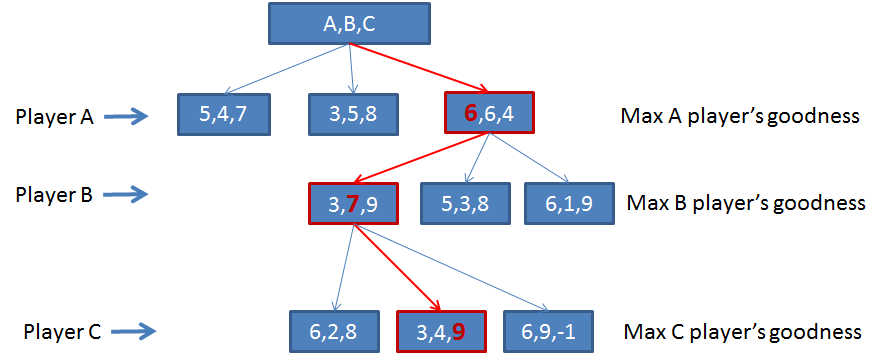
\includegraphics[width=0.9\columnwidth]{hw3_q2}\centering 
\caption{Illustrate 3 players for minimax strategy}
\end{figure}
\item  Implement $\alpha\beta$ for the game of gobblet. Assume that if a state $\sigma$ is repeated, then the game is a draw:

\begin{equation}
\forall(\sigma)\ [\textsf{move}(\textsf{move}(\sigma, \textsf{player1}),\textsf{player2}) = \sigma] \rightarrow (\textsf{game}(\sigma) := \textsf{draw})
\end{equation}

The game should be able to play: human vs. human = h2, human vs. robot = hr (human goes first),
robot vs. human (robot goes first), robot vs. robot = r2. There are two sets of parameters: Level:
beginer = 0, intermediate = 1, expert = 2. This places a limit on the depth of the search. You must
decide experimentally how this is applied; Time: $x$ min. This is the bound on the time you run $\alpha\beta.$ The main function should be called $ \textsf{gobby} (\textsf{players,level,time})$ where players $\in \{\textsf{h2,hr,rh,rr}\}$. The
output should be a sequence of moves with the final state when it's won or drawn.
\\
\\
\textsf{gobby(r2,2,2.5)}
\\
\\
 means robot versus robot, expert, no longer than two minutes and 30 seconds should elapse after the
opponent makes a move. Whatever is unspecified at this point, you must make decisions on.\\
\underline{Answer to Problem 3:}
\begin{itemize}
\item First I replace gobblet game rule with tic tac toe game rule to make it easier
\item In my implementation, there is human player and computer player, which we can choose h2,hr,or r2
\item time elapsed is showing during the game to reminder the game player, if the player can not take action within the time controller(eg, 180 seconds), then game over
\item the player level is implemented as clock.tick() which controls the running speed.
\item Full code is available in $gobby1\_jinjujiang.py$
\end{itemize}
Here it is some screen shot about game running:\\
\begin{figure}[h]
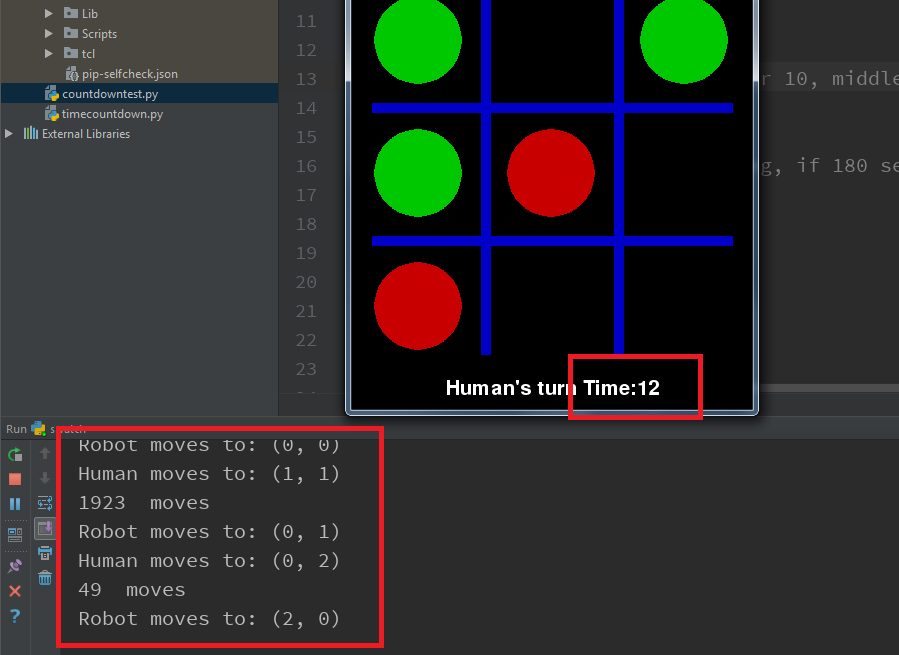
\includegraphics[width=0.9\columnwidth]{hw3_q3_1}\centering 
\caption{Illustrate human and robot game playing}
\end{figure}
\pagebreak


Here came more about Gobblet implementation:\\

\begin{itemize}
\item Then further investigate Gobblet game rule
\item The difference is how to calculate the heuristic function, and find min,max value, then using the same alpha beta pruning strategy
\item since Gobblet game rule is more complicated, the player level and game control time impacts expansions of the	game state during each turn's search. I use $MAX\_EXPAND$ which allows each player $MAX\_EXPAND$ expansions of the game state during each turn's search
\item $MAX\_EXPAND$=int(player level*time control)
\item Implement Gobblet game rule into the first implementation, then got the final solution
\item the code is available in $gobby2\_jinjujiang.py$
\end{itemize}

\end{enumerate}
\end{document}
